\part{Aspectos Gerais}

\chapter[Aspectos Gerais]{Aspectos Gerais}
\section{Aspectos Gerais}
Na indústria moderna, existem diversos métodos e técnicas disponíveis para desenvolver e colocar um produto no mercado. A escolha do método mais adequado depende de vários fatores, como o material utilizado na fabricação e a quantidade necessária para atender à demanda. Entre esses materiais, os termoplásticos têm se tornado cada vez mais populares devido à sua versatilidade e eficiência. De acordo com um relatório da Mordor Intelligence, espera-se que o mercado de termoplásticos apresente uma taxa de crescimento anual composta (CAGR) superior a 6% até 2028. Esse aumento é impulsionado pela crescente demanda por materiais leves na indústria automotiva, que busca melhorar a eficiência energética e oferecer maior flexibilidade de design.

Para a produção em larga escala de produtos feitos com termoplásticos, o processo de injeção plástica é amplamente utilizado. Esse método garante alta uniformidade das peças, além de permitir uma produção rápida e eficiente. O processo consiste em injetar o plástico, no estado líquido, em um molde que dará forma ao produto final desejado. Para isso, o molde precisa ser projetado levando em consideração diversas características do produto final, como o material escolhido, o volume de produção e os requisitos geométricos. O design do molde exige uma combinação de conhecimentos em engenharia, ciência dos materiais e uso de tecnologias avançadas, além de contemplar aspectos como material do molde, resistência térmica, propriedades do polímero, sistema de resfriamento, alimentação e ejeção.

Ferramentas de simulação computacional, como o software Moldflow, têm se tornado indispensáveis no processo de desenvolvimento de moldes. Essas tecnologias permitem prever o comportamento do material durante a injeção, analisar o fluxo do polímero e identificar possíveis problemas, como deformações, linhas de solda e pontos de estresse. Com o auxílio da simulação, os projetistas podem otimizar o design do molde antes mesmo de sua fabricação, reduzindo custos, minimizando desperdícios e diminuindo o tempo necessário para ajustes posteriores.

\section{Objetivos}

O objetivo principal deste trabalho é projetar e desenvolver um molde para injeção plástica destinado à fabricação de corpos de prova para ensaios de tração, utilizando como base os padrões definidos pela norma ISO 527. O molde será concebido para operar em uma máquina de injeção Romi Prática 80, disponível na universidade, e fabricado para atender às demandas práticas e acadêmicas da instituição.

De forma mais específica, este trabalho busca:

\begin{itemize}
    \item Estudar e compreender os fundamentos do processo de injeção plástica, com ênfase nas etapas de projeto e fabricação de moldes;
    \item Analisar os materiais termoplásticos utilizados no processo de injeção, avaliando propriedades como resistência térmica, comportamento de fluxo e encolhimento, a fim de determinar sua adequação para a fabricação dos corpos de prova;
    \item Utilizar ferramentas de simulação computacional, como o Moldflow e o Ansys, para otimizar o design do molde e prever o comportamento do material durante o processo de injeção;
    \item Modelar o molde utilizando o software SolidWorks, aproveitando suas ferramentas de CAD 3D para desenvolver uma representação detalhada e funcional do projeto;
    \item Projetar um molde funcional, considerando fatores como resistência térmica, sistema de alimentação, resfriamento e ejeção, de forma a garantir eficiência produtiva e qualidade do produto final;
    \item Validar o molde projetado, por meio de análises teóricas e simulações, antes de sua fabricação;
    \item Contribuir para a comunidade acadêmica, ao disponibilizar um modelo prático e replicável para o desenvolvimento de outros moldes e estudos na área de injeção plástica.
\end{itemize}

\section{O Processo de Desenvolvimento de Moldes}

O desenvolvimento de moldes segue uma sequência de etapas críticas, que visam garantir que o produto final seja produzido de maneira eficiente e com alta qualidade. Essas etapas envolvem uma combinação de planejamento inicial, projeto detalhado e testes finais, como mostrado no fluxograma da Figura~\ref{fig:processo_moldes}.

\begin{figure}[h]
    \centering
    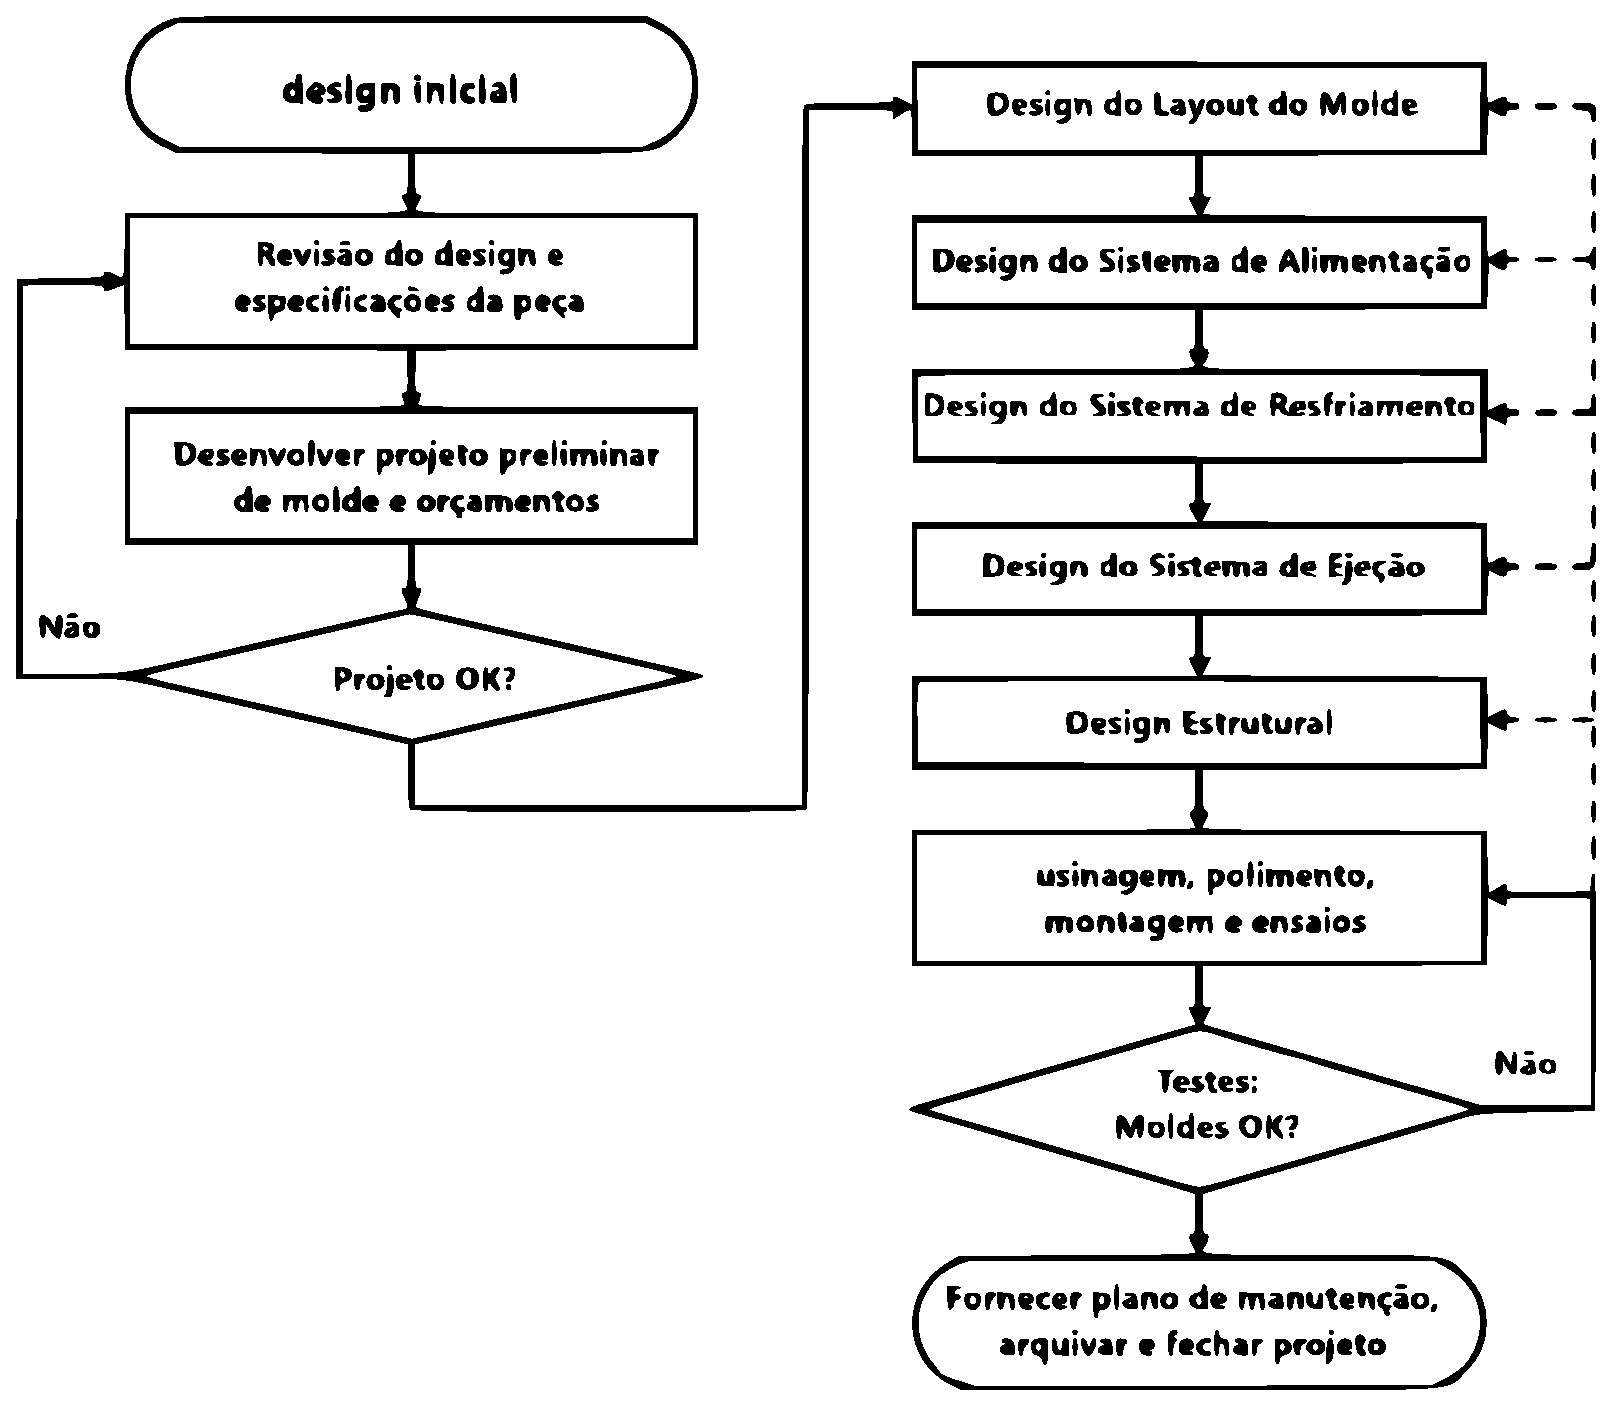
\includegraphics[keepaspectratio=true,scale=0.3]{figuras/aspectosgerais/Processo_de_criacao_de_molde.eps}
    \caption{Processo de projetar o molde}
    \label{processo_molde}
\end{figure}

O processo começa com o \textbf{design inicial}, no qual o projeto da peça é revisado, considerando suas especificações e requisitos funcionais. A partir dessa análise, são desenvolvidos projetos preliminares do molde, juntamente com orçamentos iniciais, que são posteriormente submetidos à aprovação.

Se o projeto for aprovado, o processo avança para o \textbf{design detalhado do molde}, que inclui várias etapas principais:

\begin{itemize}
    \item \textbf{Projeto do Layout do Molde (Mold Layout Design)}: Definição da estrutura geral do molde, incluindo as posições das cavidades, canais de alimentação e sistemas de ejetores.
    
    \item \textbf{Design do Sistema de Alimentação (Feed System Design)}: Planejamento dos canais pelos quais o material fundido será injetado nas cavidades do molde, assegurando que o material flua uniformemente.
    
    \item \textbf{Design do Sistema de Resfriamento (Cooling System Design)}: Determinação da disposição dos canais de resfriamento para controlar a taxa de resfriamento da peça moldada, essencial para evitar deformações.
    
    \item \textbf{Design do Sistema de Ejeção (Ejector System Design)}: Planejamento dos mecanismos de ejeção que removem as peças acabadas do molde sem danificá-las.
    
    \item \textbf{Design Estrutural (Structural System Design)}: Avaliação da integridade estrutural do molde, garantindo que ele suporte as forças de injeção e o ciclo repetitivo de aquecimento e resfriamento.
\end{itemize}




 

\section{Composição e estrutura do trabalho}

A formatação do trabalho como um todo considera três elementos principais: 
(1) pré-textuais, (2) textuais e (3) pós-textuais. Cada um destes, pode se 
subdividir em outros elementos formando a estrutura global do trabalho, 
conforme abaixo (as entradas itálico são \textit{opcionais}; em itálico e
negrito são \textbf{\textit{essenciais}}):

\begin{description}
	\item [Pré-textuais] \

	\begin{itemize}
		\item Capa
		\item Folha de rosto
		\item \textit{Dedicatória}
		\item \textit{Agradecimentos}
		\item \textit{Epígrafe}
		\item Resumo
		\item Abstract
		\item Lista de figuras
		\item Lista de tabelas
		\item Lista de símbolos e
		\item Sumário
	\end{itemize}

	\item [Textuais] \

	\begin{itemize}
		\item \textbf{\textit{Introdução}}
		\item \textbf{\textit{Desenvolvimento}}
		\item \textbf{\textit{Conclusões}}
	\end{itemize}

	\item [Pós-Textuais] \
	
	\begin{itemize}
		\item Referências bibliográficas
		\item \textit{Bibliografia}
		\item Anexos
		\item Contracapa
	\end{itemize}
\end{description}

Os aspectos específicos da formatação de cada uma dessas três partes 
principais do relatório são tratados nos capítulos e seções seguintes.

No modelo \LaTeX, os arquivos correspondentes a estas estruturas que devem
ser editados manualmente estão na pasta \textbf{editáveis}. Os arquivos
da pasta \textbf{fixos} tratam os elementos que não necessitam de 
edição direta, e devem ser deixados como estão na grande maioria dos casos.

\section{Considerações sobre formatação básica do relatório}

A seguir são apresentadas as orientações básicas sobre a formatação do
documento. O modelo \LaTeX\ \textbf{já configura todas estas opções corretamente},
de modo que para os usuários deste modelo o texto de toda esta Seção é 
\textbf{meramente informativo}.

\subsection{Tipo de papel, fonte e margens}

Papel -- Na confecção do relatório deverá ser empregado papel branco no 
formato padrão A4 (21 cm x 29,7cm), com 75 a 90 g/m2.

Fonte -- Deve-se utilizar as fontes Arial ou Times New Roman no tamanho 12 
pra corpo do texto, com variações para tamanho 10 permitidas para a 
wpaginação, legendas e notas de rodapé. Em citações diretas de mais de três 
linhas utilizar a fonte tamanho 10, sem itálicos, negritos ou aspas. Os 
tipos itálicos são usados para nomes científicos e expressões estrangeiras, 
exceto expressões latinas.

Margens -- As margens delimitando a região na qual todo o texto deverá estar 
contido serão as seguintes: 

\begin{itemize}
	\item Esquerda: 03 cm;
	\item Direita	: 02 cm;
	\item Superior: 03 cm;
	\item Inferior: 02 cm. 
\end{itemize}

\subsection{Numeração de Páginas}

A contagem sequencial para a numeração de páginas começa a partir da 
primeira folha do trabalho que é a Folha de Rosto, contudo a numeração em 
si só deve ser iniciada a partir da primeira folha dos elementos textuais. 
Assim, as páginas dos elementos pré-textuais contam, mas não são numeradas 
e os números de página aparecem a partir da primeira folha dos elementos 
textuais, que se iniciam na Introdução. 

Os números devem estar em algarismos arábicos (fonte Times ou Arial 10) no 
canto superior direito da folha, a 02 cm da borda superior, sem traços, 
pontos ou parênteses. 

A paginação de Apêndices e Anexos deve ser contínua, dando seguimento ao 
texto principal.

\subsection{Espaços e alinhamento}

Para a monografia de TCC 01 e 02 o espaço entrelinhas do corpo do texto 
deve ser de 1,5 cm, exceto RESUMO, CITAÇÔES de mais de três linhas, NOTAS 
de rodapé, LEGENDAS e REFERÊNCIAS que devem possuir espaçamento simples. 
Ainda, ao se iniciar a primeira linha de cada novo parágrafo se deve 
tabular a distância de 1,25 cm da margem esquerda.

Quanto aos títulos das seções primárias da monografia, estes devem começar 
na parte superior da folha e separados do texto que o sucede, por um espaço 
de 1,5 cm entrelinhas, assim como os títulos das seções secundárias, 
terciárias. 

A formatação de alinhamento deve ser justificado, de modo que o texto fique 
alinhado uniformemente ao longo das margens esquerda e direita, exceto para 
CITAÇÕES de mais de três linhas que devem ser alinhadas a 04 cm da margem 
esquerda e REFERÊNCIAS que são alinhadas somente à margem esquerda do texto 
diferenciando cada referência.

\subsection{Quebra de Capítulos e Aproveitamento de Páginas}

Cada seção ou capítulo deverá começar numa nova pagina (recomenda-se que 
para texto muito longos o autor divida seu documento em mais de um arquivo 
eletrônico). 

Caso a última pagina de um capitulo tenha apenas um número reduzido de 
linhas (digamos 2 ou 3), verificar a possibilidade de modificar o texto 
(sem prejuízo do conteúdo e obedecendo as normas aqui colocadas) para 
evitar a ocorrência de uma página pouco aproveitada.

Ainda com respeito ao preenchimento das páginas, este deve ser otimizado, 
evitando-se espaços vazios desnecessários. 

Caso as dimensões de uma figura ou tabela impeçam que a mesma seja 
posicionada ao final de uma página, o deslocamento para a página seguinte 
não deve acarretar um vazio na pagina anterior. Para evitar tal ocorrência, 
deve-se reposicionar os blocos de texto para o preenchimento de vazios. 

Tabelas e figuras devem, sempre que possível, utilizar o espaço disponível 
da página evitando-se a \lq\lq quebra\rq\rq\ da figura ou tabela. 

\section{Cópias}

Nas versões do relatório para revisão da Banca Examinadora em TCC1 e TCC2, 
o aluno deve apresentar na Secretaria da FGA, uma cópia para cada membro da 
Banca Examinadora.

Após a aprovação em TCC2, o aluno deverá obrigatoriamente apresentar a 
versão final de seu trabalho à Secretaria da FGA na seguinte forma:

\begin{itemize}
	\item 01 cópia encadernada para arquivo na FGA;
	\item 01 cópia não encadernada (folhas avulsas) para arquivo na FGA;
	\item 01 cópia em CD de todos os arquivos empregados no trabalho.
\end{itemize}

A cópia em CD deve conter, além do texto, todos os arquivos dos quais se 
originaram os gráficos (excel, etc.) e figuras (jpg, bmp, gif, etc.) 
contidos no trabalho. Caso o trabalho tenha gerado códigos fontes e 
arquivos para aplicações especificas (programas em Fortran, C, Matlab, 
etc.) estes deverão também ser gravados em CD. 

O autor deverá certificar a não ocorrência de “vírus” no CD entregue a 
secretaria. 

